\documentclass[utf8x, 14pt, bold, times]{G7-32} % Стиль (по умолчанию будет 14pt)

\sloppy

% Настройки стиля ГОСТ 7-32
% Для начала определяем, хотим мы или нет, чтобы рисунки и таблицы нумеровались в пределах раздела, или нам нужна сквозная нумерация.
%\EqInChapter % формулы будут нумероваться в пределах раздела
%\TableInChapter % таблицы будут нумероваться в пределах раздела
%\PicInChapter % рисунки будут нумероваться в пределах раздела

% Добавляем гипертекстовое оглавление в PDF
\usepackage[
bookmarks=true, colorlinks=true, unicode=true,
urlcolor=black,linkcolor=black, anchorcolor=black,
citecolor=black, menucolor=black, filecolor=black,
]{hyperref}

\AfterHyperrefFix

% полезный пакет для микротипографии, увы под xelatex мало чего умеет,
% но под pdflatex хорошо улучшает читаемость
\usepackage{microtype}

% Тире могут быть невидимы в Adobe Reader
\ifInvisibleDashes
\MakeDashesBold
\fi

\usepackage{graphicx}   % Пакет для включения рисунков

% С такими оно полями оно работает по-умолчанию:
% \RequirePackage[left=20mm,right=10mm,top=20mm,bottom=20mm,headsep=0pt,includefoot]{geometry}
% Если вас тошнит от поля в 10мм --- увеличивайте до 20-ти, ну и про переплёт не забывайте:

\geometry{right=10mm}
\geometry{left=30mm}
\geometry{top=20mm}
\geometry{bottom=20mm}
% считать от нижней границы текста
\geometry{ignorefoot}


% Пакет Tikz
\usepackage{tikz}
\usetikzlibrary{arrows,positioning,shadows}

% Произвольная нумерация списков.
\usepackage{enumerate}

% ячейки в несколько строчек
\usepackage{multirow}

% itemize внутри tabular
\usepackage{paralist,array}

%\setlength{\parskip}{1ex plus0.5ex minus0.5ex} % разрыв между абзацами
\setlength{\parskip}{1ex} % разрыв между абзацами
\usepackage{blindtext}

% Центрирование подписей к плавающим окружениям
%\usepackage[justification=centering]{caption}

\usepackage{newfloat}
\DeclareFloatingEnvironment[
placement={!ht},
name=Equation
]{eqndescNoIndent}
\edef\fixEqndesc{\noexpand\setlength{\noexpand\parindent}{\the\parindent}\noexpand\setlength{\noexpand\parskip}{\the\parskip}}
\newenvironment{eqndesc}[1][!ht]{%
    \begin{eqndescNoIndent}[#1]%
\fixEqndesc%
}
{\end{eqndescNoIndent}}

% Располагает все картинки (floats) до начала
% следующего раздела
\usepackage[section]{placeins}

% Двойная горизонтальная линия у таблиц
\usepackage{hhline}
% Расстояние между линиями
\setlength\doublerulesep{.5pt}

% Нумерация списка не по ГОСТУ.
% Первый уровень числа, второй - буквы
\renewcommand{\labelenumi}{\arabic{enumi})}
\renewcommand{\labelenumii}{\asbuk{enumii})}
\renewcommand{\labelitemi}{$\bullet$}

% Настройки листингов.
\usepackage{local-minted}

\usepackage{amsmath}
\makeatletter
\let\save@mathaccent\mathaccent
\newcommand*\if@single[3]{%
  \setbox0\hbox{${\mathaccent"0362{#1}}^H$}%
  \setbox2\hbox{${\mathaccent"0362{\kern0pt#1}}^H$}%
  \ifdim\ht0=\ht2 #3\else #2\fi
  }
%The bar will be moved to the right by a half of \macc@kerna, which is computed by amsmath:
\newcommand*\rel@kern[1]{\kern#1\dimexpr\macc@kerna}
%If there's a superscript following the bar, then no negative kern may follow the bar;
%an additional {} makes sure that the superscript is high enough in this case:
\newcommand*\widebar[1]{\@ifnextchar^{{\wide@bar{#1}{0}}}{\wide@bar{#1}{1}}}
%Use a separate algorithm for single symbols:
\newcommand*\wide@bar[2]{\if@single{#1}{\wide@bar@{#1}{#2}{1}}{\wide@bar@{#1}{#2}{2}}}
\newcommand*\wide@bar@[3]{%
  \begingroup
  \def\mathaccent##1##2{%
%Enable nesting of accents:
    \let\mathaccent\save@mathaccent
%If there's more than a single symbol, use the first character instead (see below):
    \if#32 \let\macc@nucleus\first@char \fi
%Determine the italic correction:
    \setbox\z@\hbox{$\macc@style{\macc@nucleus}_{}$}%
    \setbox\tw@\hbox{$\macc@style{\macc@nucleus}{}_{}$}%
    \dimen@\wd\tw@
    \advance\dimen@-\wd\z@
%Now \dimen@ is the italic correction of the symbol.
    \divide\dimen@ 3
    \@tempdima\wd\tw@
    \advance\@tempdima-\scriptspace
%Now \@tempdima is the width of the symbol.
    \divide\@tempdima 10
    \advance\dimen@-\@tempdima
%Now \dimen@ = (italic correction / 3) - (Breite / 10)
    \ifdim\dimen@>\z@ \dimen@0pt\fi
%The bar will be shortened in the case \dimen@<0 !
    \rel@kern{0.6}\kern-\dimen@
    \if#31
      \overline{\rel@kern{-0.6}\kern\dimen@\macc@nucleus\rel@kern{0.4}\kern\dimen@}%
      \advance\dimen@0.4\dimexpr\macc@kerna
%Place the combined final kern (-\dimen@) if it is >0 or if a superscript follows:
      \let\final@kern#2%
      \ifdim\dimen@<\z@ \let\final@kern1\fi
      \if\final@kern1 \kern-\dimen@\fi
    \else
      \overline{\rel@kern{-0.6}\kern\dimen@#1}%
    \fi
  }%
  \macc@depth\@ne
  \let\math@bgroup\@empty \let\math@egroup\macc@set@skewchar
  \mathsurround\z@ \frozen@everymath{\mathgroup\macc@group\relax}%
  \macc@set@skewchar\relax
  \let\mathaccentV\macc@nested@a
%The following initialises \macc@kerna and calls \mathaccent:
  \if#31
    \macc@nested@a\relax111{#1}%
  \else
%If the argument consists of more than one symbol, and if the first token is
%a letter, use that letter for the computations:
    \def\gobble@till@marker##1\endmarker{}%
    \futurelet\first@char\gobble@till@marker#1\endmarker
    \ifcat\noexpand\first@char A\else
      \def\first@char{}%
    \fi
    \macc@nested@a\relax111{\first@char}%
  \fi
  \endgroup
}
\makeatother


\begin{document}

\frontmatter % выключает нумерацию ВСЕГО; здесь начинаются ненумерованные главы: реферат, введение, глоссарий, сокращения и прочее.

\newcommand{\university}{
    Федеральное~государственное~автономное \\
    образовательное~учреждение \\
    высшего образования \\
    <<СИБИРСКИЙ~ФЕДЕРАЛЬНЫЙ~УНИВЕРСИТЕТ>>}
\newcommand{\faculty}{Институт~космических~и~информационных~технологий}
\newcommand{\department}{Кафедра~прикладной~математики~и~компьютерной~безопасности}
\newcommand{\city}{Красноярск}
\newcommand{\docname}{ОТЧЕТ~ПО~ЛАБОРАТОРНОЙ~РАБОТЕ}
\newcommand{\num}{~№2}
\newcommand{\topic}{Основы криптографии с открытым ключом. Алгоритм RSA}
\newcommand{\variant}{Вариант~№~1}
\newcommand{\tutorname}{Ю.~В.~Потылицина}
\newcommand{\studentname}{С.~А.~Абрамов}
\newcommand{\group}{КИ20-08Б}
\newcommand{\gradebook}{032049480}

\renewcommand*{\maketitle}{
\begin{titlepage}
    \thispagestyle{empty}
    \begin{center}
        \university \\
        \faculty \\
		\department \\[6cm]

        \textbf{\docname \num} \\
		\topic \\
        \variant \\[5.1cm]

        \vfill
        \setlength\extrarowheight{-2pt}
        \begin{tabular*}{\textwidth}{@{\extracolsep{\fill}} lcl}
            \normalsize{Преподаватель:} & \underline{\hspace{3cm}} & \normalsize{\tutorname} \\
                          & {\small подпись, дата} & \\
            \normalsize{Студент:}~\normalsize{\group,~\gradebook}   & \underline{\hspace{3cm}} & \normalsize{\studentname} \\
                          & {\small подпись, дата} & \\
        \end{tabular*}
        \vfill
		\city~\the\year
	\end{center}
\end{titlepage}
}

\maketitle

\newpage
\tableofcontents

\nobreakingbeforechapters
%\breakingbeforechapters

\newpage
\Introduction

\textbf{Цель работы:}
\begin{itemize}
\item ознакомиться с основами ассиметричной криптографии;
\item ознакомиться с элементами теории чисел, используемых в криптографии с
      открытым ключом;
\item изучить особенности алгоритма с открытым ключом RSA;
\item получить навыки разработки криптосистем с открытым ключом с
      использованием языка программирования высокого уровня.
\end{itemize}

\textbf{Задание на работу:}
разработать алгоритм шифрования/расшифровывания RSA, со следующими особенностями:
\begin{itemize}
\item объём исходного текста – любой (в разумных пределах);
\item исходный текст может состоять из русских и английских букв, цифр, а
      также знаков препинания;
\item исходный текст находится в кодировке ASCII (или Unicode);
\item выступающее в качестве модуля число – N, которое выбирается автоматически и
      состоит из 31 ДЕСЯТИЧНОГО знака. Числа P и Q выбираются случайным образом,
      так, что $P \cdot Q = N$, где $P$ и $Q$~–~простые числа.
\item исходный текст разбивается на K блоков, где K выбирается исходя из
      значения модуля N.
\end{itemize}

Убедиться в правильности составления алгоритмов, а затем на языке
программирования составить программу, которая реализует данный алгоритм.

На ряде контрольных примеров (не менее 10) открытого текста проверить
правильность работы алгоритмов шифрования и дешифрования.

Оценить криптостойкость данного алгоритма RSA, а также производительность,
разработанной программы.

Разработанная программа должна содержать графический интерфейс пользователя.

\mainmatter % это включает нумерацию глав и секций в документе ниже
\newpage

\chapter{Описание алгоритма}

\section{Алгоритм создания открытого и секретного ключей}

RSA-ключи генерируются следующим образом:

\begin{enumerate}
\item выбираются два различных случайных простых числа $p$ и $q$ заданного размера;
\item вычисляется их произведение $n = p \cdot q$, которое называется модулем;
\item вычисляется значение функции Эйлера от числа $n$:
      \begin{equation}
        \varphi(n) = (p − 1) \cdot (q − 1)
      \end{equation}
\item выбирается целое число $e$ $(1 < e < \varphi(n))$, взаимно простое со значением
      функции $\varphi(n)$;
\item вычисляется число $d$, мультипликативно обратное к числу $e$ по модулю $\varphi(n)$,
      то есть число, удовлетворяющее сравнению:
      \begin{equation}
        d \cdot e \equiv 1 \pmod{\varphi(n)} 
      \end{equation}
      (число $d$ называется секретной экспонентой; обычно оно вычисляется при помощи расширенного алгоритма Евклида);
\item пара $(e, n)$ публикуется в качестве открытого ключа RSA;
\item пара $(d, n)$ играет роль закрытого ключа RSA и держится в секрете.
\end{enumerate}

\section{Алгоритм шифрования}

\begin{itemize}
\item Взять открытый ключ $(e, n)$;
\item Взять открытый текст $m$;
\item Зашифровать сообщение с использованием открытого ключа:
      \begin{equation}
        c = E(m) = m^e \mod n
      \end{equation}
\end{itemize}

\section{Алгоритм расшифрования}

\begin{itemize}
\item Принять зашифрованное сообщение $c$;
\item Взять свой закрытый ключ $(d, n)$;
\item Применить закрытый ключ для расшифрования сообщения:
      \begin{equation}
        m = D(c) =c^d \mod n
      \end{equation}
\end{itemize}

\chapter{Оценка алгоритма}

Данная реализация алгоритма RSA не является \textsl{практически надёжной},
т.к. односторонняя функция $E(m)$ является \textsl{детерминированной} - при
одних и тех же значениях входных параметров (ключа и сообщения) выдаёт одинаковый
результат. Это значит, что не выполняется необходимое условие практической
(семантической) надёжности шифра.

Для решения этой проблемы можно использовать модифицированную версию функции $E(m)$:
\begin{equation}
  c = E'(m) = (m||random)^e \mod n
\end{equation}
Но это решение также имеет недостатки (См. \href{https://habr.com/ru/post/99376/}{Хабр: RSA, а так ли все просто?}).

Узкое место по производительности данной реализации - генерация полупростого числа $n$
определённой длины $l$: 
\begin{enumerate}
\item Генерируется два случайных различных числа $p$ и $q$ длиной $\frac{l}{2}$;
\item Они проверяются на простоту с помощью теста Миллера-Рабина;
\item Вычисляется $n = p \cdot q$;
\item Если длина $n$ не равна $l$, то повторяются шаги 1-3.
\end{enumerate}

\chapter{Примеры работы программы}

\section{Пример 1}

\textbf{Исходный текст:} \\
    Hello!

\textbf{Публичный ключ $(e, n)$:} \\
    (1336750571917222506367500878005, 8085472216604733526839569321341)

\textbf{Приватный ключ $(d, n)$:} \\
    (1478409329065133370310312496101, 8085472216604733526839569321341)

\textbf{Зашифрованный текст:} \\
    5807241446759901267216605390094 1945721761216314545617066200940
    1389314913534850043257468141227 1389314913534850043257468141227
    6572208100939281410200927429783 3016927945680088341886714157792
    ~~~~~~~~~~~~~~~~~~~~~~~~~~~~~~~

Результаты работы программы представлены на рисунках~\ref{ris:encode-test-1}-\ref{ris:decode-test-1}.

\vspace{\baselineskip}
\begin{figure}[H]
\center{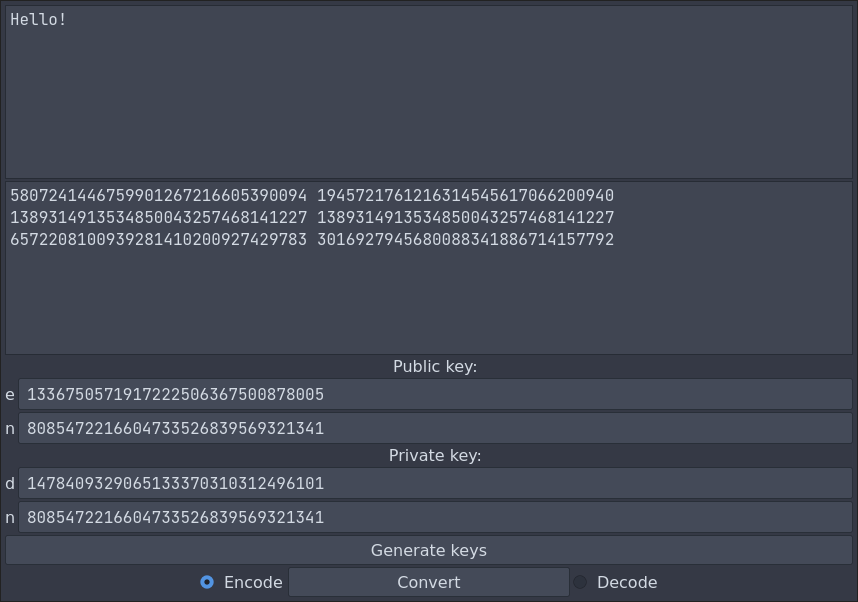
\includegraphics[width=0.8\linewidth]{figures/encode-test-1}}
    \caption{Шифрование}
\label{ris:encode-test-1}
\end{figure}

\vspace{\baselineskip}
\begin{figure}[H]
\center{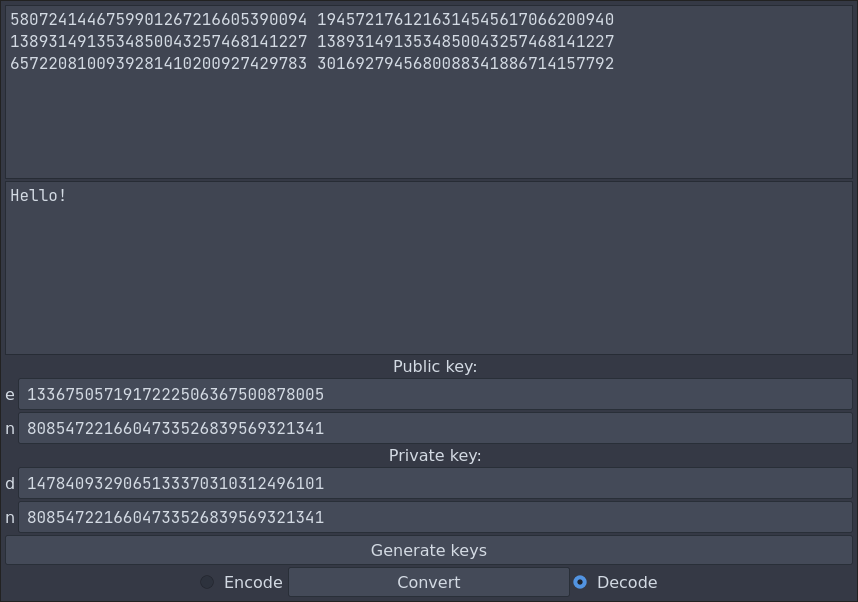
\includegraphics[width=0.8\linewidth]{figures/decode-test-1}}
    \caption{Расшифрование}
\label{ris:decode-test-1}
\end{figure}


\section{Пример 2}

\textbf{Исходный текст:} \\
    Привет!

\textbf{Публичный ключ $(e, n)$:} \\
    (5491526198967652564128883404649, 8677899933955039287323181182263)

\textbf{Приватный ключ $(d, n)$:} \\
    (6530236606095563597175180039049, 8677899933955039287323181182263)

\textbf{Зашифрованный текст:} \\
    2451790758248836813047077465653 6929963014385198466056100423531
    1792994633186142959029214273249 1068251925414506252246529379223
    6486422004695066299507395395040 4941598345502762856208188833893
    6161224323360842715260972435122

Результаты работы программы представлены на рисунках~\ref{ris:encode-test-2}-\ref{ris:decode-test-2}.

\vspace{\baselineskip}
\begin{figure}[H]
\center{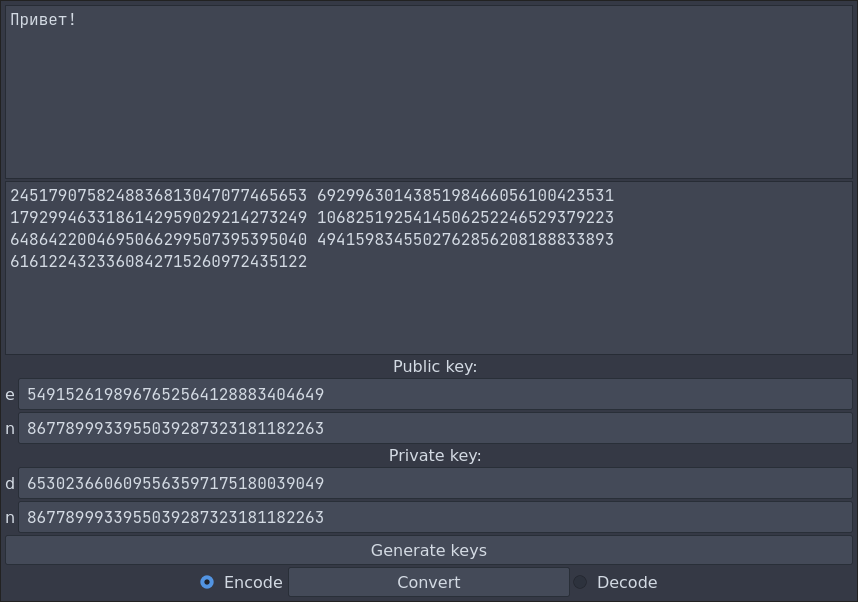
\includegraphics[width=0.8\linewidth]{figures/encode-test-2}}
    \caption{Шифрование}
\label{ris:encode-test-2}
\end{figure}

\vspace{\baselineskip}
\begin{figure}[H]
\center{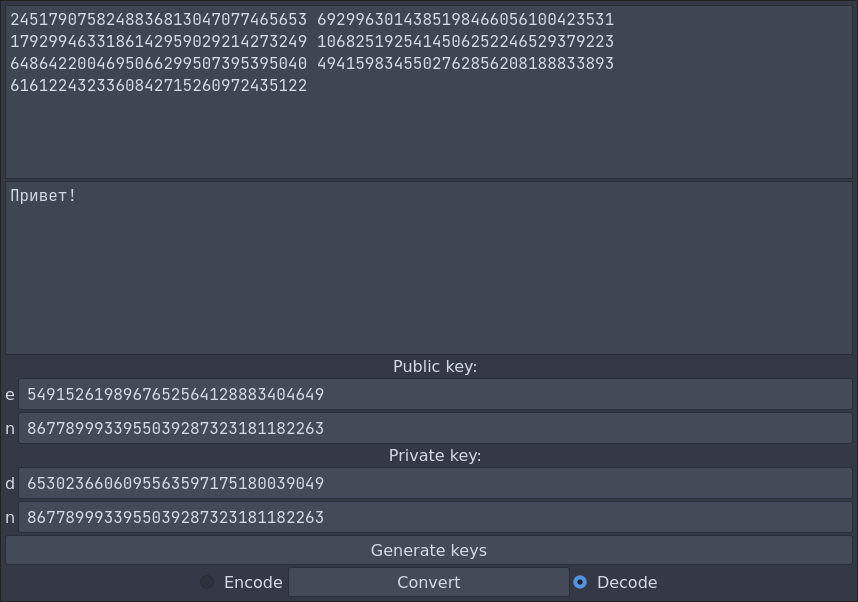
\includegraphics[width=0.8\linewidth]{figures/decode-test-2}}
    \caption{Расшифрование}
\label{ris:decode-test-2}
\end{figure}


\section{Пример 3}

\textbf{Исходный текст:} \\
    01.2022

\textbf{Публичный ключ $(e, n)$:} \\
    (5491526198967652564128883404649, 5450820981215398882735645358813)

\textbf{Приватный ключ $(d, n)$:} \\
    (5036971201715425118500854709795, 5450820981215398882735645358813)

\textbf{Зашифрованный текст:} \\
    4147457564135597823149308362883 5221272554176426416441937009602
    3535023798586647103690228134215 1928538648444993962750216906620
    4147457564135597823149308362883 1928538648444993962750216906620
    1928538648444993962750216906620 

Результаты работы программы представлены на рисунках~\ref{ris:encode-test-3}-\ref{ris:decode-test-3}.

\vspace{\baselineskip}
\begin{figure}[H]
\center{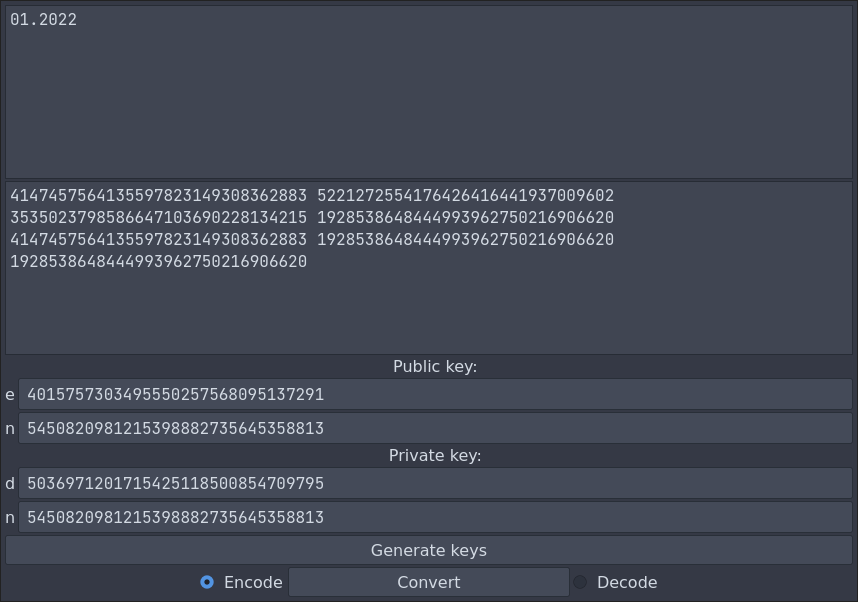
\includegraphics[width=0.8\linewidth]{figures/encode-test-3}}
    \caption{Шифрование}
\label{ris:encode-test-3}
\end{figure}

\vspace{\baselineskip}
\begin{figure}[H]
\center{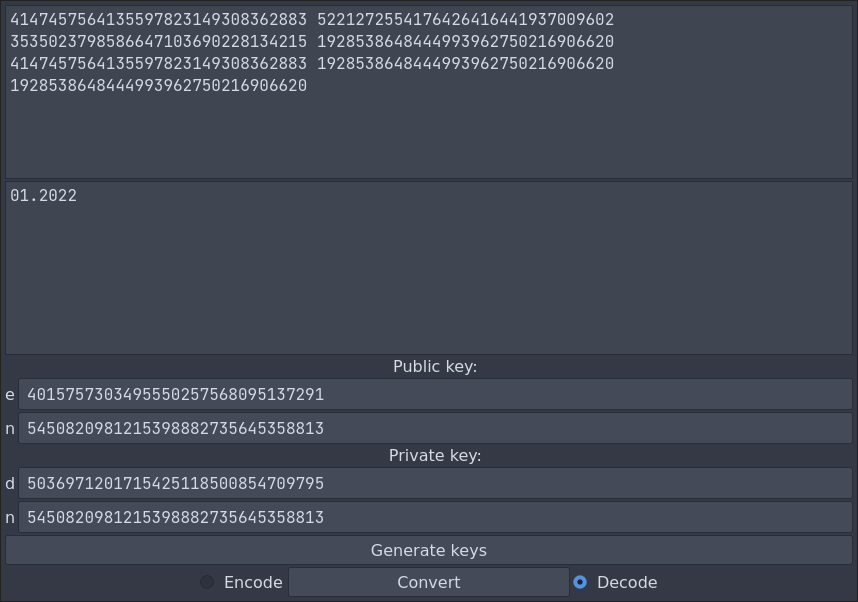
\includegraphics[width=0.8\linewidth]{figures/decode-test-3}}
    \caption{Расшифрование}
\label{ris:decode-test-3}
\end{figure}


\section{Пример 4}

\textbf{Исходный текст:} \\
    !?;,:.-

\textbf{Публичный ключ $(e, n)$:} \\
    (1827821233260228957330462119381, 8606963804773339124904139583897)

\textbf{Приватный ключ $(d, n)$:} \\
    (1618330337596630383004261807997, 8606963804773339124904139583897)

\textbf{Зашифрованный текст:} \\
    7682999861805463840962051524493 4403838174454233083555965378737
    1909354241146547364672395621626 6858093156978570257166638594841
    5048676731057660471922055344624 1308786662182323412950422448348
    8590765347481596817223057719572 

Результаты работы программы представлены на рисунках~\ref{ris:encode-test-4}-\ref{ris:decode-test-4}.

\vspace{\baselineskip}
\begin{figure}[H]
\center{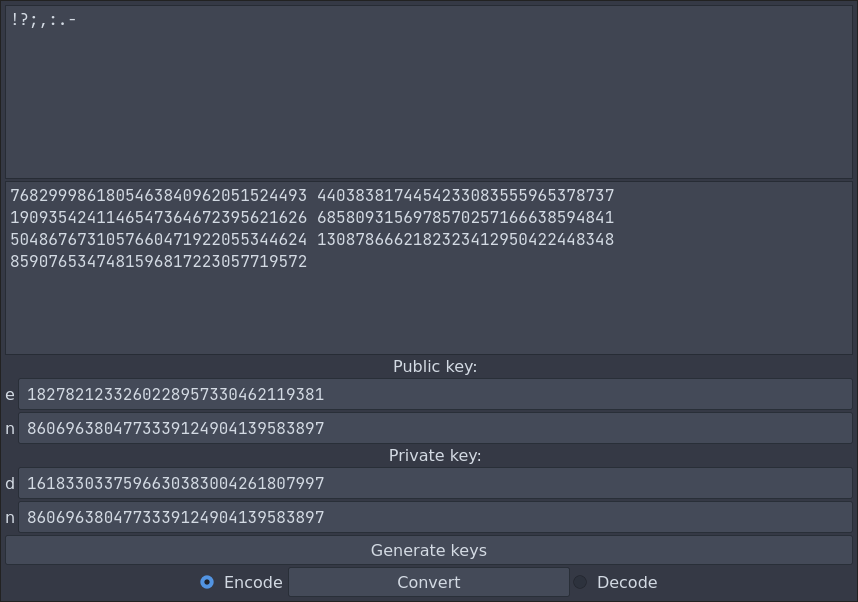
\includegraphics[width=0.8\linewidth]{figures/encode-test-4}}
    \caption{Шифрование}
\label{ris:encode-test-4}
\end{figure}

\vspace{\baselineskip}
\begin{figure}[H]
\center{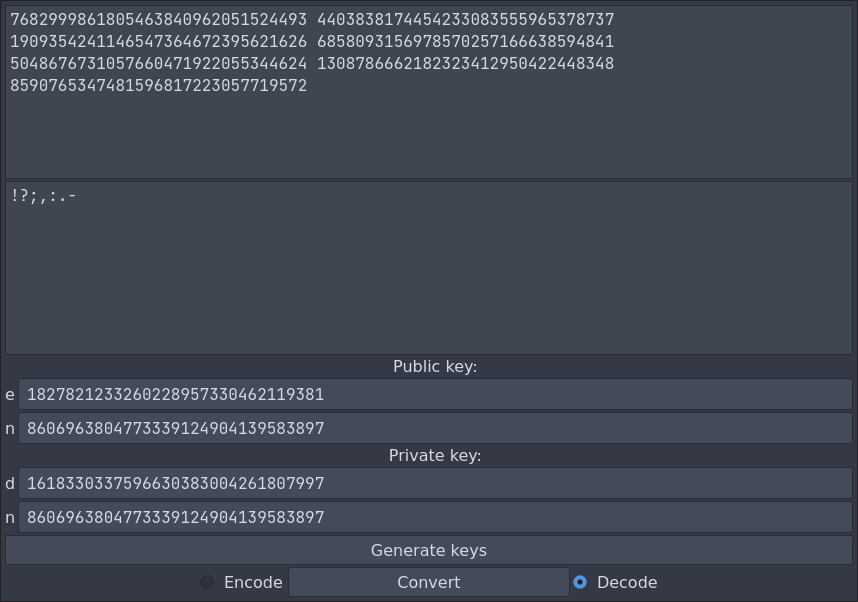
\includegraphics[width=0.8\linewidth]{figures/decode-test-4}}
    \caption{Расшифрование}
\label{ris:decode-test-4}
\end{figure}


\section{Пример 5}

\textbf{Исходный текст:} \\
    БГЯDSI!

\textbf{Публичный ключ $(e, n)$:} \\
    (1827821233260228957330462119381, 5791792681103248967722057525079)

\textbf{Приватный ключ $(d, n)$:} \\
    (2304676846327366406913727452413, 5791792681103248967722057525079)

\textbf{Зашифрованный текст:} \\
    3385608287236349261478244092696 2842962959242576787797687409723
    1026508350809114738769887424519 963820060395904968790397299828
    3789600647708532359425234605570 3104067190146191090063779640918
    1070021809437130113590398289664

Результаты работы программы представлены на рисунках~\ref{ris:encode-test-5}-\ref{ris:decode-test-5}.

\vspace{\baselineskip}
\begin{figure}[H]
\center{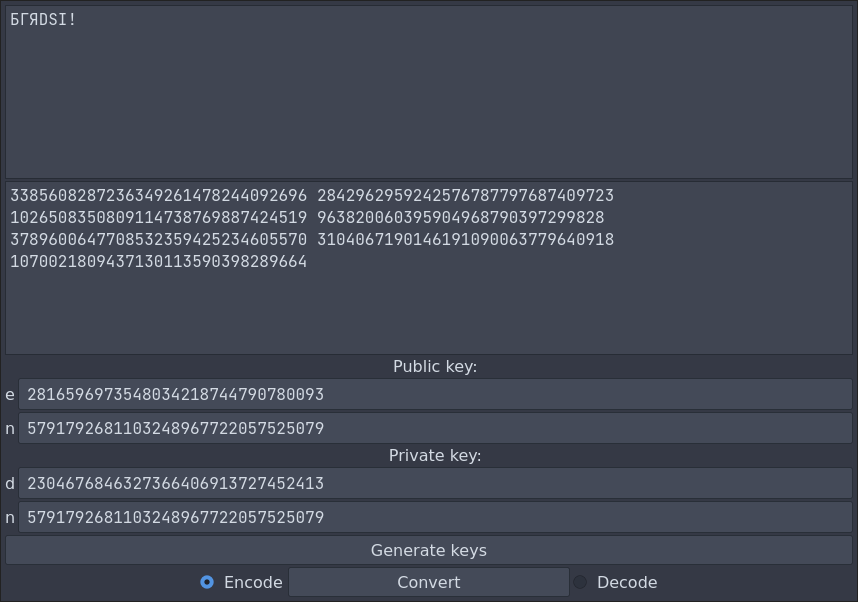
\includegraphics[width=0.8\linewidth]{figures/encode-test-5}}
    \caption{Шифрование}
\label{ris:encode-test-5}
\end{figure}

\vspace{\baselineskip}
\begin{figure}[H]
\center{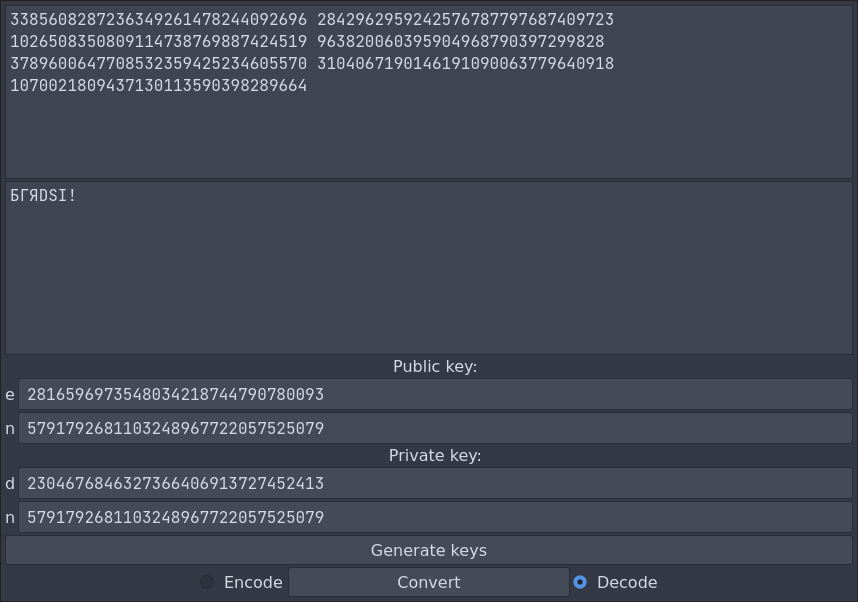
\includegraphics[width=0.8\linewidth]{figures/decode-test-5}}
    \caption{Расшифрование}
\label{ris:decode-test-5}
\end{figure}


\chapter{Исходный код}

\section{rsa\_lib.py}

\inputminted[fontsize=\footnotesize, breaklines]{python}{../../src/rsa_lib.py}
%\inputminted[linenos,frame=single,fontsize=\footnotesize,style=bw,fontfamily=cyrillicfontttnoftr]{python}{../src/rsa_lib.py}

\section{widget.py}

\inputminted[fontsize=\footnotesize, breaklines]{python}{../../src/widget.py}
%\inputminted[linenos,frame=single,fontsize=\footnotesize,style=bw,fontfamily=cyrillicfontttnoftr]{python}{../src/widget.py}

\section{ui\_widget.py}

\inputminted[fontsize=\footnotesize, breaklines]{python}{../../src/ui_widget.py}
%\inputminted[linenos,frame=single,fontsize=\footnotesize,style=bw,fontfamily=cyrillicfontttnoftr]{python}{../src/ui_widget.py}

\iffalse
Анализ граф-схемы микропрограммы (ГСМ) показал, что дополнительных пустых
операторных вершин вводить не требуется. ГСМ, размеченная для автомата Мили,
приведена на рисунке~\ref{ris:marked-graph-scheme}.

\vspace{\baselineskip}
\begin{figure}[H]
\center{\includegraphics[width=0.5\linewidth]{figures/marked-graph-scheme.png}}
    \caption{Граф-схема микропрограммы, размеченная для автомата Мили}
\label{ris:marked-graph-scheme}
\end{figure}
\fi


\backmatter %% Здесь заканчивается нумерованная часть документа и начинаются ссылки и

\newpage
\Conclusion

В ходе работы изучил ассиметричный алгоритм шифрования RSA, его недостатки и преимущества.
А также убедился, что наивная реализация алгоритма не является криптостойкой.

Узнал, что с Python 3.8+ функция pow(основание, показатель, модуль) при указанном модуле
поддерживает отрицательный показатель степени\cite{python-pow}.
С помощью этой функциональности нашел обратное по модулю целое число $d$.

\newpage
\nocite{*}
\bibliographystyle{ugost2008}
\bibliography{doc}

\end{document}
